% !TEX program = xelatex
% Cards format — auto-generated from harness-factory.tex by cards-convert.mjs
\documentclass[11pt]{article}

\usepackage{fontspec}
\usepackage{unicode-math}
% Latin Modern by OTF filename (not font name): xelatex on macOS (Core
% Text, no fontconfig) cannot resolve "Latin Modern Roman" by name, which
% silently produced ~4KB broken card PDFs. kpathsea finds the OTFs in
% texmf-dist on both macOS and the oven's Linux xelatex.
\setmainfont{lmroman10-regular.otf}[
  BoldFont=lmroman10-bold.otf,
  ItalicFont=lmroman10-italic.otf,
  BoldItalicFont=lmroman10-bolditalic.otf,
]
\setsansfont{lmsans10-regular.otf}[
  BoldFont=lmsans10-bold.otf,
  ItalicFont=lmsans10-oblique.otf,
  BoldItalicFont=lmsans10-boldoblique.otf,
]
\setmonofont{lmmono10-regular.otf}[Scale=0.88,
  BoldFont=lmmonolt10-bold.otf,
  ItalicFont=lmmono10-italic.otf,
]


\usepackage{graphicx}
\graphicspath{{figures/}{../arxiv-ac/figures/}}
\usepackage{booktabs}
\usepackage{tabularx}
\usepackage{adjustbox}
\usepackage{ragged2e}
\usepackage{microtype}
\usepackage{natbib}
\usepackage{fancyvrb}
\usepackage{balance}



\makeatletter
\def\input@path{{../}}
\makeatother
\usepackage{ac-paper-cards}
\acdraftfalse

% Extra commands from base paper
\newcommand{\code}[1]{\texttt{#1}}
\definecolor{acteal}{RGB}{42,138,130}
\usetikzlibrary{positioning,arrows.meta,fit,calc}
\fvset{fontsize=\scriptsize,frame=leftline,rulecolor=\color{acpink},framerule=1.2pt,xleftmargin=0.6em,framesep=0.6em,samepage=true}

\hypersetup{
  pdftitle={Pick the Type First},
}

\renewcommand{\acpdfbase}{pick-the-type-first-26-arxiv}
\begin{document}

% ============================================================
% TITLE CARD
% ============================================================
\thispagestyle{empty}
\vspace*{0.05em}
\begin{center}
\href{https://papers.aesthetic.computer}{
\includegraphics[height=11em]{pals-card}}\par\vspace{0.1em}
{\acbold\fontsize{18pt}{22pt}\selectfont\color{acdark} Pick the Type First}\par
\vspace{0.1em}
\vspace{0.2em}
{\scriptsize\color{acgray}\href{https://prompt.ac/@jeffrey}{\color{cyan!70!blue}\textbf{@jeffrey}}\,\textperiodcentered\,Aesthetic{\acdot}Computer\,\textperiodcentered\,ORCID~\href{https://orcid.org/0009-0007-4460-4913}{0009-0007-4460-4913}}\par
\vspace{0.2em}
\rule{0.5\textwidth}{0.5pt}\par
\vspace{0.12em}
\ifacdraft\colorbox{yellow!60}{\small\color{red!80!black}\textbf{\textit{working draft --- not for citation}}}\par
\vspace{0.1em}\fi
{\scriptsize\color{acgray} October 30, 2026 \,\textperiodcentered\, \href{https://github.com/whistlegraph/aesthetic-computer/commit/d23575e7d3}{d23575e7d3}}\par
\end{center}

% ============================================================
% INDEX CARD
% ============================================================
\cardindex

% ============================================================
% BODY
% ============================================================
\section{Introduction}
\label{sec:intro}

Ask a room of art students what an AI agent is and you get a cloud. Ask them
what it is \emph{making} and the cloud gets a shape. A poster. A sound. A
web page. That shape has a standard name already: a MIME type
\citep{rfc2045,rfc2046}.

Aesel is built on that. Its terminal shows the media a session is working
on: a module reads the paths in each tool call, keeps the ones that are real
files of a kind a card can show --- \code{image/png}, \code{audio/wav},
\code{video/mp4}, \code{application/pdf} and seven other types --- and puts the
freshest first, so the preview turns to what was just written
(\code{aesel/src/media.mjs}). Its companion, mime.ac, files everything
people post into boards by MIME type \citep{mimedoc}. The type is the shape of
the work in both places.

A harness is everything around a model that lets it act. Aesel's own is
large: sectioned prompts, guardrails, tool guidance, a verify loop, and a
refinement method borrowed from Harness$^2$ \citep{xu2026harness2,scudder2026harnessloop}.
That is too much to teach in an afternoon. The harness factory keeps the
shape and drops the size. It has four parts, inputs, a written prompt, a model
and checks, aimed at one MIME type. Choosing that type comes first, and it
sets most of what follows.

This report describes the factory as committed at \code{d23575e7d3}
(October 30, 2026), the runs made with it that day, and the workshop it was
built for. The commit is evidence. The classroom is still a plan.

\section{Context}
\label{sec:context}

\textbf{Harnesses, not weights.} Harness$^2$ \citep{xu2026harness2}
improves an agent by editing its harness. Twelve days before this commit,
that method was carried over to Aesel \citep{scudder2026harnessloop,aeselharnessdoc}:
the prompt moved into named markdown sections, a runner played every save in
a headless browser, and a refinement loop proposed edits. The factory is the
same idea for beginners. The editable part is one file, \code{prompt.md},
and the loop is a person reading \code{runs/}.

\textbf{Formats as culture.} Sterne reads the MP3 as a cultural object that
encodes assumptions about listening \citep{sterne2012mp3}. Menkman reads file
formats as having vernaculars of their own \citep{menkman2010vernacular}.
Keymaps as Social Software, written for the same UCLA program, treated a
keyboard layout as a score that people share and version \citep{scudder2026keymaps}.
The factory comes at it from the other side: a format can be picked
\emph{first}, as the constraint a whole tool is designed around.

\textbf{The room.} The workshop is written for UCLA Design Media Arts, where
the Social Software initiative \citep{sosoft_info} ran its second cycle,
\emph{Scores for Social Software} \citep{reas2026scores}, in spring 2026.
The published sub-platter for that cycle \citep{sosoftplatter} gathers its
paper, edition and documentation. Its lesson for this one is practical:
students there wrote scores, instructions for other people to perform. A
\code{prompt.md} is a score for a model.

\textbf{Low floor, wide walls.} Resnick and Silverman ask construction kits
for a low floor, a high ceiling and wide walls \citep{resnick2005reflections},
after Papert \citep{papert1980mindstorms}. Here the floor is one command
from a starter. The walls are the 3 input forms $\times$ 10 output goals.
The ceiling is the fact that Aesel's own harness has the same shape at a much
larger size.

\section{The factory}
\label{sec:factory}

\subsection{A harness is a folder}
\begin{Verbatim}
my-harness/
  harness.json  {"name","inputs":["text","image"],
                 "output":"image/svg+xml","model"?}
  prompt.md     what it knows, how it decides
  check.mjs     optional: (output) => [problems]
  runs/         every run, kept
\end{Verbatim}
Inputs come in three forms: \code{text} on the command line, \code{image}
(any picture file, sent as a PNG) and \code{file} (a text file up to 64\,KB,
read in as words). A harness refuses a form its manifest did not name, so
that a run means what \code{harness.json} says. The model defaults to
hosted Claude Sonnet~5.5; \code{--model} swaps it. Four commands drive it:
\code{ac harness list}, \code{new}, \code{run} and \code{post}
(\code{aesel/src/harness-cli.mjs}, 116 lines; the factory itself is
\code{harness-factory.mjs}, 337).

\subsection{The goal decides}
Table~\ref{tab:goals} is the \code{OUTPUTS} registry, close to verbatim. One
line per MIME type. Each line fixes the extension, the contract appended to
the student's prompt, the checks a result must pass, and how the answer
becomes bytes. A student who writes \code{--out wav} has chosen all of that
in one word.

\begin{table}[t]
\centering
\scriptsize
\setlength{\tabcolsep}{2pt}
\begin{adjustbox}{max width=\linewidth,center}%
\begin{tabularx}{\linewidth}{@{}l l l X@{}}
\toprule
Goal & Ext & Route & Built-in check \\
\midrule
\code{text/plain} & txt & answer & not empty \\
\code{text/markdown} & md & answer & not empty \\
\code{text/csv} & csv & answer & not empty \\
\code{application/json} & json & answer & parses \\
\code{text/html} & html & answer & has an \code{<html>} element \\
\code{image/svg+xml} & svg & answer & one complete \code{<svg>}…\code{</svg>} \\
\code{text/x-lisp} & lisp & answer & parentheses balance \\
\code{text/javascript} & mjs & answer & source checks; no imports;\newline exports \code{paint} \\
\code{image/png} & png & \textbf{art-direct} & prompt under 16{,}000 chars \\
\code{audio/wav} & wav & \textbf{score} & bpm 20--300; real pitches; $\le$60\,s \\
\bottomrule
\end{tabularx}%
\end{adjustbox}
\caption{The ten output goals. \emph{Answer}: the model's fenced block
is the file. \emph{Art-direct}: the block is a prompt sent to a hosted image
model. \emph{Score}: the block is JSON this machine synthesizes. A
\code{check.mjs} adds its own problems after the built-in ones pass.}
\label{tab:goals}
\end{table}

The seam is visible. \code{ac harness run --dry} prints exactly what would
be sent and spends nothing. For the poster starter:
\begin{Verbatim}
# Poster
You design one Swiss-style typographic poster
for the event you're given.
- Canvas: viewBox="0 0 600 900".
- ...
- Use only generic font families
  (sans-serif, serif, monospace).
---
Output goal: image/svg+xml (picture).
Answer with one standalone SVG document (with
xmlns and a viewBox) inside one ```svg block.
No external images or fonts.
--- user ---
late night jazz at the planetarium, nov 14
\end{Verbatim}
Everything above the rule is the student's. Everything below it is the
type's. The workshop teaches that line: you write taste and judgement, and
the factory adds the format.

\subsection{Three routes to bytes}
Eight goals are text, and the model writes the file. The other two are the
lesson inside the lesson (Figure~\ref{fig:flow}). A language model emits
tokens. It cannot emit a PNG's pixels or a WAV's samples. So the harness
picks an intermediate form the model \emph{can} write, and something else
turns it into the media.

For \code{image/png} the model is the art director. Its contract asks for
\emph{subject, composition, medium, palette, light and mood in concrete
words}, under 1,500 characters, and the hosted image model paints it. If a
photo came in, it goes along as a reference. For \code{audio/wav} the model
is the composer. It writes \code{\{"bpm", "notes": [\{"at", "beats",
"pitch", "wave", "gain"\}]\}}, and \code{wav-score.mjs} sings it. That file
has one voice per note, five waveforms (sine, square, saw, triangle,
noise), a short attack and release against clicks, and a \code{tanh} soft
clip into 16-bit mono at 22,050\,Hz. It has no dependencies, so a workshop
laptop needs nothing new. The synth is plain on purpose. The score carries
the music.

\begin{figure*}[t]
\centering
\resizebox{!}{0.86\textheight}{\rotatebox{90}{\begin{tikzpicture}[
  font=\sffamily\scriptsize,
  box/.style={draw=acdark, fill=white, rounded corners=2pt, align=center, minimum height=9mm, inner sep=3pt, text width=#1},
  box/.default=20mm,
  you/.style={draw=acpink, fill=acpink!10, rounded corners=2pt, align=center, minimum height=9mm, inner sep=3pt, text width=20mm},
  mod/.style={draw=acpurple, fill=acpurple!10, rounded corners=2pt, align=center, minimum height=9mm, inner sep=3pt, text width=20mm},
  rt/.style={draw=acteal, fill=acteal!8, rounded corners=2pt, align=center, minimum height=6.5mm, inner sep=2pt, text width=30mm},
  goal/.style={draw=acpink, fill=acpink!25, rounded corners=3pt, align=center, minimum height=7mm, inner sep=3pt, font=\sffamily\scriptsize\bfseries},
  arr/.style={-{Stealth[length=1.6mm]}, draw=acdark, line width=0.5pt},
  dec/.style={-{Stealth[length=1.4mm]}, draw=acpink, dashed, line width=0.5pt}]
% main row
\node[box] (in) {inputs\\ \code{text} \code{image} \code{file}};
\node[you, right=5mm of in] (prompt) {\code{prompt.md}\\ + contract};
\node[mod, right=5mm of prompt] (model) {hosted model\\ (braincells)};
\node[box, right=5mm of model] (check) {extract +\\ checks};
\node[rt, right=7mm of check, yshift=8.5mm] (r1) {answer \emph{is} the file};
\node[rt, right=7mm of check] (r2) {prompt $\rightarrow$ image model};
\node[rt, right=7mm of check, yshift=-8.5mm] (r3) {score $\rightarrow$ local synth};
\node[box, right=7mm of r2] (file) {\code{runs/<time>/}\\ \code{output.<ext>}};
\node[box, right=8mm of file] (board) {mime.ac\\ board by type};
% goal: a banner across the top, straight drops to what it decides
\coordinate (gl) at ($(prompt.west)+(0,21mm)$);
\coordinate (gr) at ($(board.east)+(0,27mm)$);
\node[goal, fit=(gl)(gr), inner sep=0pt] (g) {};
\node[font=\sffamily\scriptsize\bfseries, text=acdark] at (g.center) {output MIME goal, named once in \code{harness.json}};
% flow
\draw[arr] (in) -- (prompt);
\draw[arr] (prompt) -- (model);
\draw[arr] (model) -- (check);
\draw[arr] (check.east) -- ++(2.5mm,0) |- (r1.west);
\draw[arr] (check.east) -- (r2.west);
\draw[arr] (check.east) -- ++(2.5mm,0) |- (r3.west);
\draw[arr] (r1.east) -- ++(2.5mm,0) |- (file.west);
\draw[arr] (r2.east) -- (file.west);
\draw[arr] (r3.east) -- ++(2.5mm,0) |- (file.west);
\draw[arr] (file) -- node[above=1pt, font=\sffamily\scriptsize] {\code{post}} (board);
% repair
\draw[arr, draw=acpink] (check.south) -- ++(0,-6mm) -| node[pos=0.25, below, text=acpink, align=center] {problems go back, once} (model.south);
% decides
\draw[dec] (g.south -| prompt) -- node[right, text=acpink] {contract} (prompt.north);
\draw[dec] (g.south -| check) -- node[right, text=acpink] {checks} (check.north);
\draw[dec] (g.south -| r1) -- node[right, text=acpink] {route} (r1.north);
\draw[dec] (g.south -| file) -- node[right, text=acpink] {extension} (file.north);
\draw[dec] (g.south -| board) -- node[right, text=acpink] {board} (board.north);
\end{tikzpicture}}}
\caption{One run of a factory harness, read bottom to top. The MIME goal (pink banner) sets the contract, checks, route, extension and board.}
\label{fig:flow}
\end{figure*}

\subsection{Checks and one repair}
A check is how a harness gets stricter without retraining anything. After the
model answers, the fenced block is pulled out (or the whole answer, when the
fence was forgotten). The type's built-in checks run, then the harness's own
\code{check.mjs}. If either returns problems, they go back to the model as a
list, and it gets one try to send the whole answer again. The terminal shows
\code{repairing:} with the first problem. Two rounds is the hard limit. The
haiku starter's check is the whole idea in four lines:
\begin{Verbatim}
export default function check({ text }) {
  const lines = text.split("\n").filter((l) => l.trim());
  return lines.length === 3 ? []
    : [`A haiku has 3 lines; this has ${lines.length}.`];
}
\end{Verbatim}

\subsection{Runs are kept}
Every run writes a timestamped folder: \code{answer.md} (the model's full
reply), \code{run.json} (inputs, model, rounds, problems, token usage) and,
when it passed, \code{output.<ext>}. Image runs also keep \code{prompt.txt},
and sound runs keep \code{score.json}. The intermediate form is saved next to
what it became. Comparing two \code{runs/} folders after changing one line of
\code{prompt.md} is the workshop's main move. \code{ac harness post} sends the
newest file to mime.ac as the signed-in handle, and it lands on the board
for its type.

\section{Hosted bounds}
\label{sec:bounds}

Inference is \ac{}'s own hosted endpoint, paid in braincells by the handle
that runs it \citep{scudder2026strangers}. Nothing else needs installing,
and no student needs an API key. The endpoint sets the edges of the factory:
\begin{itemize}
\item \textbf{Words and PNGs only.} The server refuses documents, audio,
video and image URLs. An image must be a static base64 PNG, at most
768$\times$768, at most 700,000 base64 characters, and at most 16 per request
(\code{system/backend/easel-input-images.mjs}). Audio, video and PDFs cannot go
\emph{in} yet. A \code{file} input is text.
\item \textbf{Billing.} Every model is billed in braincells against a daily
allowance that resets at midnight UTC; an exhausted handle gets a 429 with
its count (\code{easel-policy.mjs}).
\item \textbf{Five pictures a day.} Hosted image generation is capped at five
per handle per day (\code{easel-image.mjs}). This
is the one goal a student should choose knowingly.
\item \textbf{8,000 output tokens} per request, set by the factory.
\end{itemize}

Two fixes came from the first live runs. \textbf{One retry.} The lab Wi-Fi
reset connections. A request that never got an answer is now tried once more
after 1.5\,s. An HTTP error is not retried, because it already has a reason.
\textbf{Shrink to fit.} A textured photograph at 768\,px can encode past the
700,000-character cap. Pictures are now box-filtered and re-encoded at 80\%
of the previous side until the PNG is under 500\,KB, giving up below 64\,px. The
factory decodes plain 8-bit PNGs itself and sends everything else (JPEG,
HEIC, WebP, 16-bit or palette PNG) through macOS's \code{sips} first.

\section{Evidence}
\label{sec:evidence}

\subsection{Live runs}
On October 30, 2026, four starters ran against hosted Claude Sonnet~5.5,
signed in as @jeffrey (Table~\ref{tab:runs}). Each passed its checks on the
first round. The run records are the source for every number below. None of
the four outputs was posted.

\begin{table}[t]
\centering
\footnotesize
\setlength{\tabcolsep}{3pt}
\begin{adjustbox}{max width=\linewidth,center}%
\begin{tabularx}{\linewidth}{@{}l X r r r@{}}
\toprule
Starter & In $\rightarrow$ out & Rnd & Out tok & Think \\
\midrule
poster & text $\rightarrow$ \code{image/svg+xml} & 1 & 2{,}016 & 952 \\
hum & text $\rightarrow$ \code{audio/wav} & 1 & 5{,}982 & 2{,}409 \\
haiku-cam & image + text $\rightarrow$ \code{text/plain} & 1 & 520 & 485 \\
kidlisp & text $\rightarrow$ \code{text/x-lisp} & 1 & 550 & 298 \\
\bottomrule
\end{tabularx}%
\end{adjustbox}
\caption{The four live runs, one each, from their \code{run.json}. \emph{Out
tok} is the output tokens billed, and \emph{Think} is the part of those spent
thinking. Inputs were 253, 354, 704 and 365 tokens. The poster took about
24\,s. The \code{image/png} starter was not run, to spare the five-a-day cap.}
\label{tab:runs}
\end{table}

\textbf{Poster.} Input: \emph{late night jazz at the planetarium, nov 14}.
The answer is a 2.1\,KB SVG: navy field, an amber planet with a tilted orbit,
a giant \emph{14}, and two four-column rows of small type on a grid
(Figure~\ref{fig:made}, left).

\textbf{Haiku cam.} Input: the Aesel pencil drawing of a donkey at an easel,
plus the words \emph{quiet studio}. Output:
\begin{quote}\small\itshape
the pink heart still wet\\
behind him, a door creaks wide\\
someone holds their breath
\end{quote}
It is 5/7/5, it names one concrete thing in the picture (the heart on the
canvas), and it leans past the frame, which is what the prompt asked. The
check confirmed only that it has three lines.

\textbf{Hum.} Input: \emph{the walk home after the first rain in LA}.
The model wrote 91 notes at 84\,bpm over 48 beats: a triangle melody built
from one three-note motif, sine pads, a saw bass and twenty noise hits
(Figure~\ref{fig:roll}). The synth rendered 34.5\,s (1,523,070 bytes). The
score is 5.8\,KB of JSON and cost 3,573 visible output tokens.

\textbf{KidLisp.} Input: \emph{fireflies over a dark pond}. One round:
\begin{Verbatim}
(wipe "black")
(ink "navy")
(box 0 (/ height 2) width (/ height 2))
(wiggle 6)
(ink "yellow")
(circle (+ 60 (* 20 (sin (/ frame 20)))) (/ height 4) 3)
...                 ; 12 lines in all, four colours
\end{Verbatim}

\begin{figure}[t]
\centering
\begin{minipage}[b]{0.43\columnwidth}\centering

\includegraphics[width=\linewidth]{poster}
\end{minipage}\hfill
\begin{minipage}[b]{0.53\columnwidth}\centering

\includegraphics[width=\linewidth]{aesel-pencil}\\[0.4em]
{\footnotesize\itshape the pink heart still wet\\ behind him, a door creaks wide\\ someone holds their breath\par}
\end{minipage}
\caption{Left: the poster run's SVG, rasterized at 1200$\times$1800 with no
edits. Right: the haiku-cam input image (Aesel's pencil donkey) and the
haiku the run wrote from it. Both were made in one round.}
\label{fig:made}
\end{figure}

\begin{figure*}[t]
\centering
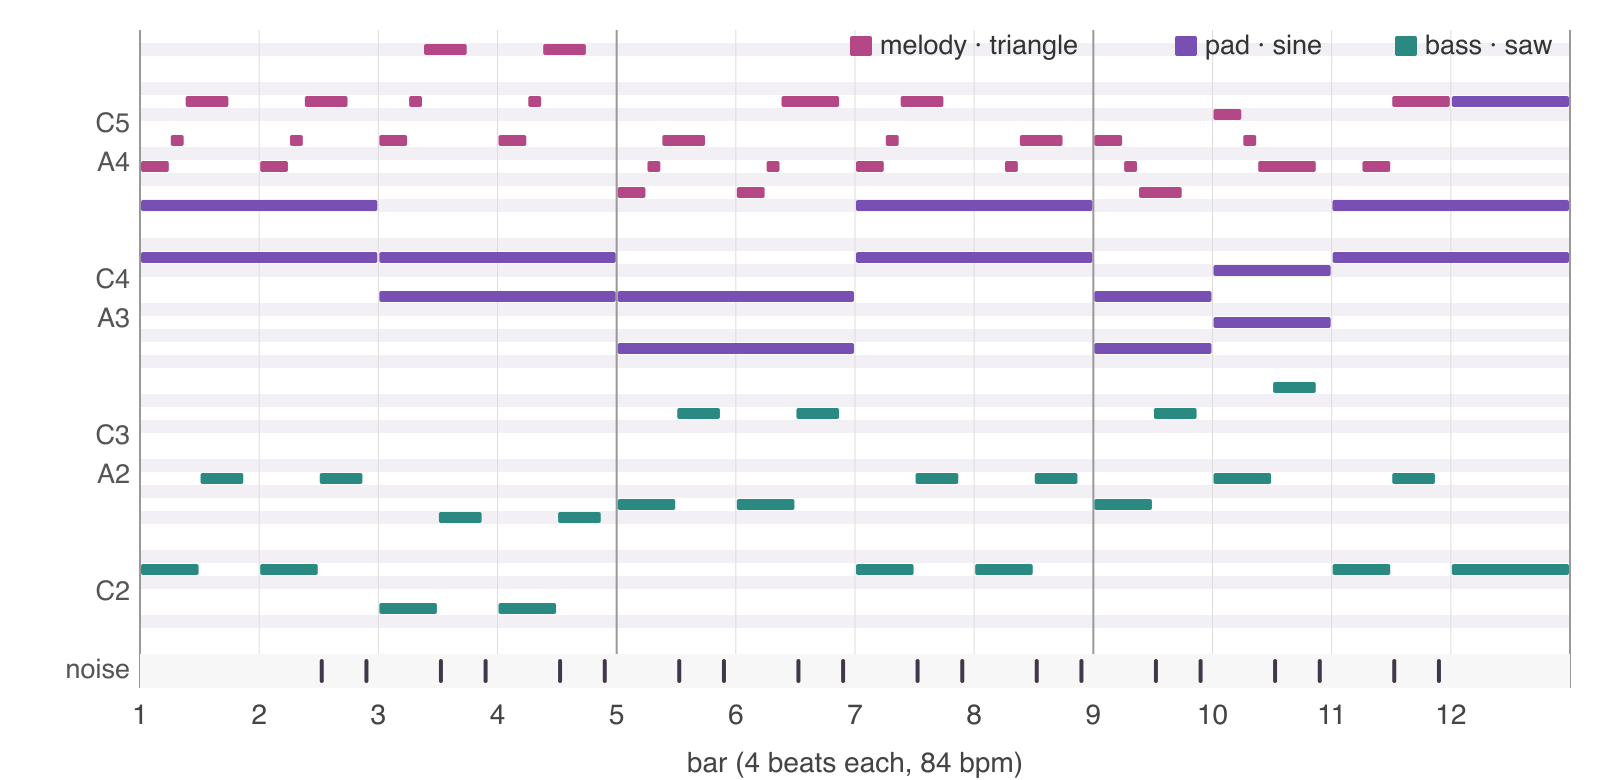
\includegraphics[width=\linewidth]{hum-roll}
\caption{The JSON score the \code{hum} run wrote, drawn as a piano roll from
its \code{score.json} (\code{figures/roll.mjs}). Twelve bars at 84\,bpm. The
melody repeats a three-note figure and shifts it, the pads hold chords, the
bass moves in octaves, and the noise lane is a light off-beat pulse. That
follows the starter's prompt: \emph{repeat a motif, then change it once}. The
local synth turned these 91 notes into a 34.5\,s WAV.}
\label{fig:roll}
\end{figure*}

\subsection{What the runs show}
\textbf{The intermediate form works on the first try.} The two goals the
model cannot reach directly are the ones this paper is about. The sound
route passed its checks first time, with a score that reads as music on paper
(Figure~\ref{fig:roll}). The picture route was exercised only by the test
suite this time, with an injected painter.

\textbf{A rule without a check is a suggestion.} The poster prompt says
\emph{use only generic font families}. The SVG set
\code{"Helvetica, Arial, sans-serif"}, with a generic family only as the
fallback. The KidLisp prompt says \emph{under 12 lines}, and the piece has
exactly 12. Neither broke anything, and no check caught either. That is the
workshop's 1:10 step in one example. If a rule matters, write it as a check
and the model gets one chance to meet it.

\textbf{The score is verbose.} A JSON note costs about 39 output tokens.
Under the 8,000-token cap, minus thinking, a score tops out around 150 notes,
far below the synth's 2,000. Most students will hit the 60-second limit
before the note limit, but a dense drum part would hit the token limit first.

\textbf{The tests.} \code{aesel/test/harness-factory.test.mjs} has 12 tests,
and all 12 pass. They cover starters as valid harnesses, refused inputs,
image bounding (1600$\times$800 in, 768$\times$384 out), the prompt seam,
per-type checks, one repair round, a score to a valid RIFF/WAVE, an
art-directed prompt passed to an injected painter, and a failed run that
keeps its answer and writes no file. Inference and painting are injected
there, so the suite spends nothing.

\section{The workshop}
\label{sec:workshop}

\code{aesel/workshop/README.md} is the route. \code{guide.html} is the same
route as a page to put on the projector. The goal is that by minute 90 every
person has written a harness, run it, changed it after watching it fail, and
posted what it made under their own handle (Table~\ref{tab:route}).

\begin{table}[t]
\centering
\footnotesize
\setlength{\tabcolsep}{3pt}
\begin{adjustbox}{max width=\linewidth,center}%
\begin{tabularx}{\linewidth}{@{}r X@{}}
\toprule
Min & Step \\
\midrule
0 & Install Aesel, \code{ac login}, \code{ac whoami} \\
10 & Run someone else's harness: everyone runs \code{poster} on their own event; three go on the projector. Why do they differ? \\
20 & Read it: \code{--dry} shows the seam between \code{prompt.md} and the contract \\
30 & Change one thing in \code{prompt.md}; compare two \code{runs/} folders; swap with a partner \\
45 & Make your own: pick an input $\times$ output pair no starter does; run it, then try to break it \\
70 & Add a \code{check.mjs}; watch \code{repairing:} \\
80 & \code{ac harness post}; walk the mime.ac boards by type \\
\bottomrule
\end{tabularx}%
\end{adjustbox}
\caption{The 90-minute route. Six starters cover the space: \code{haiku-cam}
(image + text $\rightarrow$ text, with a check), \code{poster} (text
$\rightarrow$ SVG), \code{zine} (text + image + file $\rightarrow$ HTML),
\code{hum} (text $\rightarrow$ WAV), \code{kidlisp} (text $\rightarrow$
KidLisp) and \code{sticker} (text + image $\rightarrow$ PNG).}
\label{tab:route}
\end{table}

The route ends on mime.ac on purpose. Because posts are filed by type, the
class's SVGs land together and the WAVs land together. Thirty harnesses built
on one decision get shown grouped by that decision. Walking the boards is the
critique.

The README also tells the instructor what to check before class: claimed
handles, a braincell allowance covering about twenty Sonnet runs per
person, the five-image cap, the room's Wi-Fi, and a folder of spare photos.
Its \emph{Going further} section points up the ceiling. Students can try a
cheaper model on the same harness, pick another image model, fork a
classmate's folder in git, or open Aesel's own \code{harness/*.md} to see the
same shape at full size.

\section{Limitations and ethics}
\label{sec:limits}

\textbf{It has not been taught.} Everything above is a system and four runs
by its author. No student has installed it, run out of time at minute 45, or
picked a pair the factory handles badly. Whether 90 minutes is enough is
unknown. The route is a plan, and this paper does not claim it works in a
room.

\textbf{Planned evaluation.} After the first session we will collect, with
consent, each harness folder and its \code{runs/}. That gives a direct
count of who reached each step (ran a starter, edited a prompt, made a new
harness, added a check, posted) and how many runs and repairs each took. We
will also ask one open question at the end: \emph{what does the MIME type
decide?} We will compare the answers with the thesis here. The posts on
mime.ac are a public record of the output, but they do not show what anyone
learned.

\textbf{One run each.} Every result in Table~\ref{tab:runs} is a single
sample from one model. First-round passes say the contracts are clear enough
for Sonnet~5.5. They say nothing about a cheaper model, which the README
invites students to try.

\textbf{Checks are shallow.} Built-in checks test form: the JSON parses, the
SVG closes, the parentheses balance. A poster can pass and be ugly, and a
score can pass and be tuneless. Judgement stays with the student, which is
intended, but the word \emph{passed} should not be read as \emph{good}.

\textbf{Platform catch.} Only macOS converts JPEG and HEIC. On Windows and
Linux an image input must already be an 8-bit PNG, and the error says so.
A mixed-laptop classroom will hit this.

\textbf{Small debris.} A run folder is made before the request goes out, so
a request that throws (a dropped connection, an oversized image) leaves an
empty folder in \code{runs/}. The workspace behind this paper has seven of
them from the attempts that preceded the two fixes. \code{post} skips them,
but a student comparing runs will see them.

\textbf{Consent and cost.} Every input, including a student's photo, goes to
the inference vendor, as in ordinary hosted use. Posting is public and
signed with the handle, and it happens only when the student runs
\code{post}. Inference is paid from the student's braincells, so a
classroom depends on that allowance or a top-up. No student data was used
here. The image in Figure~\ref{fig:made} is \ac{}'s own artwork.

\section{Conclusion}
\label{sec:conclusion}

A harness is inputs, a written prompt, a model and checks, aimed at one kind
of media. Name the kind and most of the rest follows: the format the model
must answer in, what counts as a broken answer, the file it becomes, and
where it gets shown. When the kind is out of the model's reach, the
harness finds a form the model can write and lets something else make the
bytes. An art director and a painter. A composer and a synth.

That is small enough to teach in an afternoon, and the same shape as the
agent tools students already use. The code is done and four runs worked on
the first try. The classroom is the next step, and it is the real test.

\vspace{0.6em}
\noindent{\footnotesize\color{acgray}\textbf{Platter consulted.} \code{papers/SCORE.md};
the public Platter index and the \code{sosoft-cycle2} sub-platter;
\emph{Edit the Harness, Not the Model}, \emph{Keymaps as Social Software},
\emph{Shipping the Easel} and their bibliographies; Aesel at
\code{d23575e7d3} (\code{harness-factory.mjs}, \code{harness-cli.mjs},
\code{wav-score.mjs}, \code{media.mjs}, \code{mime.mjs}, the workshop and its
tests); \code{MIME.md}, \code{easel-input-images.mjs},
\code{easel-policy.mjs}, \code{easel-image.mjs}; and the four run folders.\par}

\balance
\bibliographystyle{plainnat}
\bibliography{references}

\end{document}
